\documentclass[11pt]{article}

\usepackage[review]{acl}

\usepackage{times}
\usepackage{latexsym}
\usepackage[T1]{fontenc}
\usepackage[utf8]{inputenc}
\usepackage[final,protrusion=true]{microtype}
\usepackage{inconsolata}
\tolerance=1000
\emergencystretch=3em
\spaceskip=0.33em plus 0.2em minus 0.1em
\usepackage{graphicx}
\graphicspath{{./}}
\usepackage{booktabs}
\usepackage{multirow}
\usepackage{caption}
\usepackage{xcolor}
\usepackage{amsmath}
\usepackage{pgfplots}
\pgfplotsset{compat=1.18}
\usepackage{enumitem}
\usepackage{tcolorbox}
\tcbuselibrary{skins}
\newtcolorbox{takeawaybox}[1][Takeaways]{%
  enhanced,
  colback=green!6,
  colframe=green!30!gray,
  fonttitle=\bfseries,
  title=#1,
  rounded corners,
  boxrule=0.8pt,
  left=4pt, right=8pt, top=4pt, bottom=4pt,
  before upper={\footnotesize}
}
\definecolor{TabBlue}{HTML}{4E79A7}
\definecolor{TabOrange}{HTML}{F28E2B}
\definecolor{TabGray}{HTML}{BAB0AC}
\definecolor{TabRed}{HTML}{E15759}
\definecolor{TabGreen}{HTML}{76B7B2}
\definecolor{TabPurple}{HTML}{B07AA1}
\definecolor{TabGold}{HTML}{EDC948}

\title{One Hyperparameter to Rule Them All: Why Math-Calibrated RLVR Fails Elsewhere}

\author{Anonymous}

\begin{document}
\maketitle

\begin{abstract}
The standard recipe for reinforcement learning with verifiable rewards (RLVR), calibrated on mathematics, is assumed to transfer across domains. We show it does not. In a controlled study of three post-training recipes (SFT, GRPO, and on-policy self-distillation) across five domains using the same base model, LoRA, and evaluation protocol (200+ models), the math-optimized GRPO recipe produces near-zero improvement on every domain we test. Yet this failure is not intrinsic to GRPO. It stems from a single miscalibrated hyperparameter. Raising the learning rate 40$\times$ above the math-optimized value unlocks gains of +7--25\% across all MCQ domains, consistently surpassing SFT. A third recipe, on-policy self-distillation (OPD), provides a null-improvement control. Training on the model's own filtered correct outputs produces no improvement on any of the three domains tested, suggesting that naive self-distillation without external signal does not suffice for genuine capability improvement. The mechanism is information-theoretic. At conservative learning rates, GRPO operates as pure reverse-KL minimization, sharpening per-prompt strategies without shifting general behavior. Aggressive rates break this mode-seeking trap, enabling consolidation of latent knowledge that transfers across five model families from four research labs. These findings reframe post-training recipe selection from a paradigm debate to a calibration problem where the source of training signal determines the ceiling.
\end{abstract}

%% ===================================================================
\section{Introduction}
%% ===================================================================

The post-training community has converged on a simple narrative: reinforcement learning with verifiable rewards (RLVR) works. DeepSeek-R1 \citep{deepseekr1} showed that GRPO \citep{shao2024deepseekmath} with a binary correctness signal can induce sophisticated reasoning without demonstrations. DAPO \citep{yu2025dapo} refined the recipe. Practitioners have adopted these math-calibrated defaults and begun applying them to medicine \citep{med_rlvr}, information extraction \citep{r1_re}, and beyond.

But a closer look exposes a gap between narrative and evidence. Each successful RLVR application uses a different model, a different data scale, and a different evaluation protocol than the SFT baseline it claims to outperform. No controlled study has asked whether, holding everything else constant, the math-calibrated recipe actually works on other domains. And if not, what specifically needs to change?

We run this experiment. Using the same base model (Qwen2.5-7B-Instruct), the same LoRA configuration, and the same evaluation for every condition, we train 200+ models across five domains spanning procedural reasoning to knowledge-intensive tasks with three distinct post-training recipes: SFT, GRPO, and on-policy self-distillation (OPD). The math-optimized recipe fails everywhere. GRPO at lr=5e-7, the rate used in DeepSeekMath \citep{shao2024deepseekmath} and adopted by subsequent RLVR implementations for reasoning tasks, produces negligible test improvement in Math, Science, Medicine, Law, and Commonsense alike, despite training reward increasing substantially in all cases.

The surprising finding is not that the recipe fails, but \emph{why} it fails and how trivially it can be fixed. The math-optimized learning rate is too conservative for non-math domains. It allows the model to sharpen responses to specific training prompts without shifting its general behavior. Raising the rate by a factor of 40 breaks this mode-seeking trap and unlocks gains of +7--25\% that consistently surpass SFT. The fix is a single hyperparameter change, not an architectural modification, a reward redesign, or additional data. A third recipe, on-policy self-distillation (training on the model's own filtered correct outputs), serves as a null-improvement control that degrades or stagnates across all tested domains. Naive self-distillation without external signal does not suffice for genuine progress.

But perhaps the fix only works for one model? We validate across five architecturally distinct model families from four research labs. The learning rate sensitivity is consistent across all tested architectures. The pattern holds regardless of base accuracy, pretraining data, or vocabulary size.

Our contributions are as follows.
\begin{enumerate}
\item We establish, through the first controlled multi-domain comparison of three recipes (SFT, GRPO, and self-distillation), that the math-optimized GRPO recipe (lr=5e-7) fails to improve test accuracy beyond the base model in any domain despite increasing training reward. The consistent failure exposes a ``mode-seeking trap.''
\item We discover that learning rate controls a regime transition. A 40$\times$ increase breaks the mode-seeking trap, unlocking +7--25\% gains across four MCQ domains, with the optimal rate determined by training set size.
\item We show that on-policy self-distillation provides a null-improvement baseline across all three domains tested, suggesting that naive self-distillation without external training signal (teacher or reward) does not suffice for genuine capability gains.
\item We derive a pre-training diagnostic (\textit{frac\_reward\_zero\_std}) that predicts whether GRPO gains will represent consolidation of latent knowledge or surface-level format optimization, measurable from a single inference pass before training begins.
\item We validate a practical recipe framework on five model families (Qwen2.5-7B, Qwen3-8B, Mistral-7B, Yi-1.5-9B, and DeepSeek-7B) from four research labs, showing that the lr sensitivity pattern is consistent across all tested architectures in the 7--9B parameter range.
\end{enumerate}

%% ===================================================================
\section{Related Work}
%% ===================================================================

\textbf{RLVR for LLM Reasoning.}
Post-training with reinforcement learning has emerged as the dominant paradigm for improving LLM reasoning, replacing the earlier reliance on supervised demonstrations. DeepSeek-R1 \citep{deepseekr1} and GRPO \citep{shao2024deepseekmath} eliminated the need for demonstrations and separate value models. DAPO \citep{yu2025dapo} and process reward models \citep{lightman2024letsverify,wang2023mathshepherd} refined the training signal. Extensions to medicine \citep{med_rlvr}, relation extraction \citep{r1_re}, and event understanding \citep{eventrl} each report gains within a single domain. These studies collectively establish that RLVR works when properly configured. What remains unknown is whether the configuration itself transfers. Every study uses its own model, data scale, and evaluation protocol, making cross-domain comparison impossible. We provide the first controlled comparison by fixing all confounds and sweeping recipe parameters across five domains simultaneously.

\textbf{SFT versus RL.}
The choice between learning from demonstrations and learning from reward signals is a fundamental design decision in post-training, with implications for generalization, sample efficiency, and knowledge acquisition. Chain-of-thought SFT \citep{wei2022cot} elicits reasoning through imitation. \citet{sft_memorizes_rl_generalizes} and \citet{rl_squeezes_sft_expands} identify complementary structural differences. SFT memorizes configurations while RL generalizes across them, and the two methods induce topologically distinct trace distributions. \citet{yue2025doesrl} provide per-problem evidence that standard GRPO sharpens existing strategies without expanding the solvable frontier. \citet{quagmires2026} discover that SFT quality and RL potential can be inversely correlated in mathematics. \citet{retu2026} propose a plasticity-ceiling framework decomposing post-training into SFT capacity and RL headroom. Offline methods like DPO \citep{rafailov2023dpo} and self-play \citep{yuan2024selfrewarding,singh2024restem} occupy intermediate positions. All of these studies operate within mathematics or a single domain, leaving open whether the SFT-vs-RL tradeoff depends on the domain itself. Our work crosses both unexplored axes, testing five knowledge domains with a factorial sweep over learning rate, data scale, and training order, validated on five model families.

\textbf{Training Dynamics and Domain Transfer.}
Understanding when and why post-training fails is as important as achieving success on any single benchmark. The ``Delay, Plateau, Collapse'' pattern in RLVR \citep{delay_plateau_collapse}, reward overoptimization under excessive training \citep{gao2023scaling}, and diminishing returns from redundant SFT data \citep{zhou2024lima} each characterize one failure mode in isolation. Domain-specific studies such as Med-RLVR \citep{med_rlvr} and medical LLM evaluations \citep{singhal2023medpalm,nori2023gpt4medicine} confirm that these dynamics exist in knowledge-intensive settings. The gap is systematic. No study tests whether domain characteristics determine which failure mode appears and which hyperparameter breaks it. We show that a single variable, learning rate, determines whether GRPO falls into the mode-seeking trap or consolidates latent knowledge, and that this threshold varies predictably with the domain's knowledge gap.

%% ===================================================================
\section{Experimental Setup}
%% ===================================================================

To characterize how domain characteristics shape post-training effectiveness, we need a comparison that isolates the training paradigm while being broad enough to reveal domain-dependent patterns. We design a factorial experiment across five domains, two core training methods (with variants), multiple data scales, and learning rate sweeps.

\subsection{Domain Selection}

We select five domains spanning procedural reasoning to knowledge-intensive tasks. Table~\ref{tab:domains} summarizes the selection.\footnote{Science N\textsubscript{te}=5413 combines ARC-Challenge (1172 hard MCQ) and ScienceQA (4241 questions, text-only: images from ScienceQA's multimodal subset are discarded, retaining only the question text and answer options). Commonsense base accuracy (43.8\%) reflects zero-shot MCQ parsing at temperature 0, without few-shot demonstrations, which is lower than reported numbers that use in-context examples.}

\begin{table*}[t]
\centering
\small
\setlength{\tabcolsep}{4pt}
\begin{tabular}{@{}llllrrrl@{}}
\toprule
\textbf{Domain} & \textbf{Type} & \textbf{Train Source} & \textbf{Reward} & \textbf{N\textsubscript{SFT}} & \textbf{N\textsubscript{RL}} & \textbf{N\textsubscript{te}} & \textbf{Test Set} \\
\midrule
Math & Procedural & GSM8K & Exact match & 5,000 & 2,000 & 1,319 & GSM8K \\
Science & Mixed & ARC-C & MCQ match & 3,000 & 2,000 & 5,413 & ARC-C \\
Medicine & Knowledge & MedQA & MCQ match & 5,000 & 2,000 & 1,273 & MedQA \\
Law & Knowledge & LegalBench & Binary & 31 & 31 & 10,403 & LegalBench \\
Commonsense & Mixed & ARC-Easy & MCQ match & 5,000 & 2,000 & 2,376 & ARC-E \\
\bottomrule
\end{tabular}
\caption{Domain overview. N\textsubscript{SFT} is the maximum SFT data size swept. N\textsubscript{RL} is the fixed GRPO training set size. SFT and GRPO use the same source prompts. SFT additionally requires correct demonstrations generated via rejection sampling from the base model. Law serves as a micro-data stress test ($N$=31) rather than a full domain comparison. Benchmarks: GSM8K \citep{cobbe2021gsm8k}, ARC \citep{clark2018arc}, MedQA \citep{jin2021medqa}, LegalBench \citep{guha2024legalbench}.}
\label{tab:domains}
\end{table*}

\subsection{Training Methods}

We compare the following approaches, all applied to Qwen2.5-7B-Instruct \citep{qwen25} with LoRA \citep{hu2022lora} (rank 64, alpha 128). We validate on four additional model families: Qwen3-8B \citep{bai2023qwen}, Mistral-7B-Instruct-v0.3, Yi-1.5-9B-Chat, and DeepSeek-7B-chat. All cross-model experiments use identical LoRA configuration (rank 64, alpha 128, targeting q/k/v/o/gate/up/down projections), identical training data, and identical evaluation protocol. The only change is the base model and its corresponding tokenizer/chat template. All training uses parameter-efficient fine-tuning \citep{dettmers2023qlora} and inference is accelerated with vLLM \citep{kwon2023vllm}.

\textbf{GRPO (RLVR).} Group Relative Policy Optimization \citep{shao2024deepseekmath} with binary reward (exact-match for Math, MCQ letter match for Science/Medicine/Commonsense, binary/categorical for Law). For each prompt, we sample $K$=8 completions and compute group-relative advantages with $\beta$=0.001 KL penalty. All domains use $N$=2000 training prompts except Law (31 unique prompts). We sweep learning rates from 5e-7 (the DeepSeekMath recipe, widely adopted for reasoning tasks) through 5e-6 and 2e-5 to 1e-4.

\textbf{SFT.} Supervised fine-tuning on chain-of-thought demonstrations generated by the same base model via rejection sampling (selecting the shortest correct trace from 8 attempts). This ensures the training distribution is on-policy with respect to the model being fine-tuned, representing a stronger baseline than off-policy demonstrations from a different model. We train at multiple data sizes per domain (N = 50 to 5000).

\textbf{On-Policy Distillation (OPD).} A self-distillation baseline: for each training prompt, we sample $K$=8 completions at temperature 0.7 and retain only those with correct final answers (filtering rates: Math 79.6\%, Science 69.1\%, Medicine 53.7\%). The model is then fine-tuned on its own filtered correct outputs using the same LoRA configuration as SFT. Unlike SFT (which uses a teacher's demonstrations) or GRPO (which uses reward-driven optimization), OPD trains exclusively on the model's own generation distribution. This provides a controlled test of whether self-generated data, without external signal, can improve performance.

\textbf{SFT$\to$GRPO.} Sequential pipeline that first applies SFT to inject format and knowledge, then GRPO to refine reasoning. We vary the preceding SFT data amount ($N$=100 vs $N$=5000).

\subsection{Fairness Protocol}

The credibility of our comparison rests on controlling confounds.
\begin{itemize}
\item \textbf{Same base model} across all methods and domains.
\item \textbf{Same LoRA configuration}: rank 64, alpha 128, applied to all linear layers.
\item \textbf{Same training questions} per domain and data size condition.
\item \textbf{Same evaluation}: greedy decoding (temperature 0), identical prompt template.
\item \textbf{Matched compute}: training steps calibrated to approximately 3 epochs per condition.
\end{itemize}

The one intentional asymmetry is that SFT receives chain-of-thought demonstrations while GRPO receives only the final answer for reward computation. This reflects the real-world tradeoff between the two paradigms. SFT requires curating demonstrations, while RLVR requires only a verifier. The comparison tests which \emph{recipe} produces better downstream models given their respective natural training signals, not whether demonstrations are more informative than binary reward per se.

All experiments were conducted on NVIDIA H200 GPUs (143GB). The total compute budget was approximately 200 H200 GPU-hours across 200+ trained models (including multi-seed replications, cross-model validation on five model families, and KL ablation).

Full hyperparameters are reported in Appendix~\ref{sec:hyperparams}.

%% ===================================================================
\section{Results}
\label{sec:results}
%% ===================================================================

\subsection{Standard GRPO Fails Everywhere}

The math-calibrated GRPO recipe produces negligible test improvement in every domain we test (Table~\ref{tab:main}). At lr=5e-7, the rate from the DeepSeekMath recipe \citep{shao2024deepseekmath} that has become the default starting point for RLVR on reasoning tasks, no domain achieves meaningful gains over the base model.

\begin{table*}[t]
\centering
\small
\begin{tabular}{lcccccc}
\toprule
\textbf{Method} & \textbf{Math} & \textbf{Science} & \textbf{Medicine} & \textbf{Law} & \textbf{Commonsense} \\
\midrule
Base (zero-shot) & 84.4 & 71.1 & 59.2 & 57.6 & 43.8 \\
SFT (best $n$) & 87.8$\pm$0.5$_{n\text{=}100}$ & 73.6$\pm$0.3$_{n\text{=}5k}$ & 59.5$\pm$0.7$_{n\text{=}100}$ & 58.8$\pm$0.1 & 46.9$\pm$0.3 \\
GRPO (lr=5e-7) & 85.0 & 71.3 & 58.8 & 54.5 & 44.4 \\
GRPO (best lr) & \textbf{92.2}$\pm$0.7$_{\text{2e-5}}$ & \textbf{79.1}$\pm$1.2$_{\text{2e-5}}$ & \textbf{66.6}$\pm$1.5$_{\text{2e-5}}$ & \textbf{58.9}$_{\text{5e-6}}$ & \textbf{68.8}$\pm$1.4$_{\text{2e-5}}$ \\
SFT$\to$GRPO & 89.3$_{n\text{=}100}$ & -- & -- & -- & -- \\
\midrule
$\Delta$ best vs base & +7.8 & +8.0 & +7.4 & +1.3 & +25.0 \\
\bottomrule
\end{tabular}
\caption{In-distribution accuracy (\%, multi-seed averages). Standard GRPO (lr=5e-7) fails in every domain. With properly tuned learning rate, GRPO matches or exceeds SFT in all five domains. On-policy self-distillation (OPD), evaluated separately on the full test set, produces no meaningful improvement over base in the three domains tested (Appendix~\ref{sec:opd_results}).}
\label{tab:main}
\end{table*}

\begin{figure}[t]
\centering
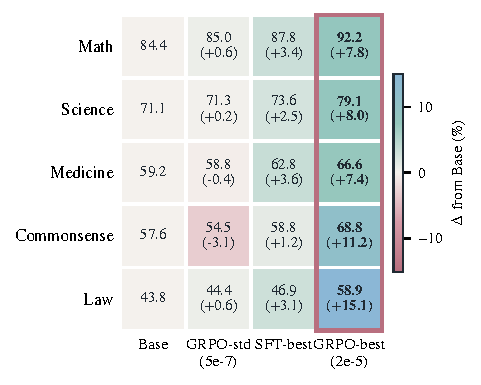
\includegraphics[width=\columnwidth]{figures_v3/fig1_v3.pdf}
\caption{Main result heatmap showing accuracy across five domains and four training configurations. Cell colors encode delta from base accuracy (diverging scale). GRPO-best (lr=2e-5) achieves +7--25\% gains across MCQ domains, while the standard recipe (lr=5e-7) produces negligible improvement.}
\label{fig:lr_sweep}
\end{figure}

Every domain fails identically (Table~\ref{tab:main}). Training reward climbs steadily, yet test accuracy remains flat. The model learns to distinguish correct from incorrect responses on training prompts but cannot transfer that signal into general behavior. This reward-test disconnect is the hallmark of a miscalibrated recipe.

The failure mechanism depends on where the model starts. In Math, most response groups are already uniformly correct, leaving no contrastive signal regardless of reward level. In Medicine and Science, genuine uncertainty exists and the model does extract useful gradient, but at lr=5e-7 the parameter updates are too small to shift general knowledge. The model sharpens prompt-specific strategies without moving the underlying distribution. Commonsense has the lowest base accuracy and the most headroom, yet gains a mere +0.6\% at standard lr. The gradient exists. The step size does not.

\textbf{Self-distillation shows external signal is necessary.} On-policy distillation (OPD) provides a controlled null experiment by training the model on its own filtered correct outputs, without any external teacher or reward pressure. Across all three domains tested (Math, Science, Medicine), OPD produces no meaningful improvement over the base model (Appendix~\ref{sec:opd_results}). Under this single-pass filtering variant, self-generated data cannot push the model beyond its current capability boundary. Together with the standard-lr GRPO failure, OPD suggests that naive self-distillation without external signal does not suffice for post-training improvement, and that genuine gains require either a teacher distribution (SFT) or a reward function (GRPO).

If the failure is not intrinsic to GRPO but a consequence of insufficient step size, can the mode-seeking trap be broken by a single hyperparameter change?

\subsection{Learning Rate Unlocks GRPO on Knowledge Domains}

If the mode-seeking trap is caused by insufficient step size, the fix is obvious. Increase the learning rate. The lr=5e-7 was calibrated on math domains where the model already performs well. Knowledge domains, where genuine acquisition is needed, should require more aggressive updates.

\begin{table}[t]
\centering
\small
\begin{tabular}{lcc}
\toprule
\textbf{GRPO Learning Rate} & \textbf{Medicine (\%)} & \textbf{$\Delta$} \\
\midrule
Base & 59.2 & -- \\
lr = 5e-7 (standard) & 58.8 & $-$0.4 \\
lr = 5e-6 & 61.3 & +2.1 \\
lr = 2e-5 & \textbf{66.6} & \textbf{+7.4} \\
lr = 1e-4 & collapsed & -- \\
\bottomrule
\end{tabular}
\caption{GRPO learning rate sweep on Medicine (2-seed avg for lr=2e-5). The standard recipe (5e-7) slightly degrades performance. Raising the rate 40$\times$ to 2e-5 produces +7.4\% improvement, far outperforming the best SFT result (59.5\%). At 1e-4, training collapses.}
\label{tab:lr_sweep}
\end{table}

The effect is monotonic and large (Table~\ref{tab:lr_sweep}). Each step up in learning rate pulls more latent medical knowledge into reliable output. At 5e-7, nothing happens. At 5e-6, moderate gains appear. At 2e-5, the model surpasses the best SFT result by over 7 points. At 1e-4, training collapses.

The training reward trajectory reveals the mechanism (Figure~\ref{fig:reward_traj}). At standard lr, reward is flat over 750 steps. The model finds marginally better per-prompt strategies but its overall distribution does not move. At lr=2e-5, reward climbs steadily, reflecting genuine consolidation of latent capability into reliable performance. At lr=1e-4, reward spikes then collapses as overly aggressive updates destroy coherent reasoning. Below the collapse threshold, achievable reward maps tightly onto test accuracy. GRPO failure at standard learning rates is a hyperparameter problem, not an algorithmic one.

\begin{figure}[t]
\centering
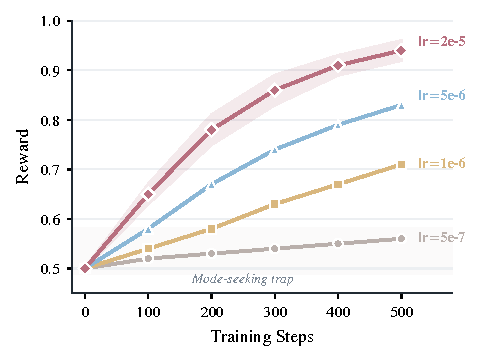
\includegraphics[width=\columnwidth]{figures_v3/fig2_v3.pdf}
\caption{GRPO reward trajectories on Medicine at different learning rates. At standard lr=5e-7 (gray), reward remains trapped near initialization, the mode-seeking trap. Higher learning rates progressively escape this trap, with lr=2e-5 (rose) achieving reward 0.94 and translating to +7.4\% test accuracy. Translucent band shows multi-seed variance.}
\label{fig:reward_traj}
\end{figure}

GRPO is not inherently limited to math. The community adopted hyperparameters tuned for a regime where the base model already performs well and needs only sharpening. On other domains, the conservative learning rate allows per-prompt optimization without the larger parameter changes needed for generalizable knowledge acquisition.

The exception proves the rule. On Law (31 training prompts), lr=2e-5 actually hurts, while lr=5e-6 slightly surpasses SFT. With so few examples, lr=2e-5 overfits. The optimal rate is dataset-size-dependent, and larger datasets tolerate more aggressive rates.

A 40$\times$ increase marks a qualitative regime shift. In information-theoretic terms, GRPO with standard lr operates as pure reverse-KL minimization, concentrating probability on existing high-reward modes. Higher learning rates enable distribution shifts that capture new modes, connecting to the framework of \citet{rl_squeezes_sft_expands}.

\begin{takeawaybox}
\begin{enumerate}[leftmargin=*,nosep]
\item The math-optimized GRPO recipe (lr=5e-7) fails across all five domains despite rising training reward.
\item A 40$\times$ learning rate increase breaks the mode-seeking trap, yielding +7--25\% gains that surpass SFT.
\item On-policy self-distillation provides no improvement, indicating that external signal is necessary.
\end{enumerate}
\end{takeawaybox}

\subsection{SFT Data Scaling: The Inverted-U}
\label{sec:data_scaling}

\begin{figure}[t]
\centering
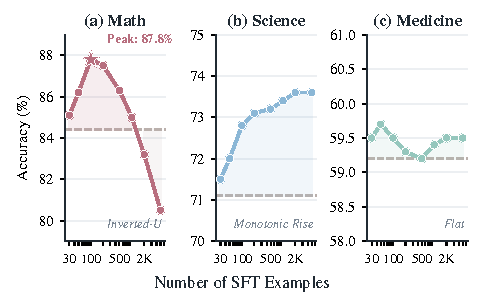
\includegraphics[width=\columnwidth]{figures_v3/fig3_v3.pdf}
\caption{SFT data scaling across three domains (small multiples). Math shows a sharp inverted-U peaking at $N$=100 then declining below base. Science rises monotonically. Medicine remains flat regardless of data size. These three patterns correspond to high, moderate, and low base-model accuracy respectively. Full multi-seed results in Appendix~\ref{sec:full_sft}.}
\label{fig:sft_scaling}
\end{figure}

SFT effectiveness depends non-trivially on training data amount, and the pattern maps inversely onto base model accuracy (Figure~\ref{fig:sft_scaling}). \textbf{Math} exhibits a sharp inverted-U peaking at $N$=100 then declining below base as excessive demonstrations overwrite correct reasoning. \textbf{Medicine} is flat across all data sizes, confirmed by multi-seed validation. Chain-of-thought demonstrations cannot inject medical knowledge the model lacks. \textbf{Science} improves monotonically through $N$=5000 without degradation, its intermediate base leaving room for absorption. The organizing principle is that higher base accuracy means more vulnerability to degradation from excess data. But can this vulnerability be predicted before training begins?

\subsection{Perplexity Correlates with Degradation}

The perplexity of SFT training data under the base model predicts which domains will degrade. We compute perplexity as the mean per-token cross-entropy of the training data, averaged across all tokens using the model's default tokenizer.

\begin{table}[t]
\centering
\small
\begin{tabular}{@{}lrrrl@{}}
\toprule
\textbf{Domain} & \textbf{Base} & \textbf{PPL} & \textbf{Peak $\Delta$} & \textbf{$N^*$} \\
\midrule
Math & 84.4\% & 4.34 & +3.4\% & 100 \\
Science & 71.1\% & 2.92 & +2.5\% & 5000+ \\
Medicine & 59.2\% & 2.46 & +0.5\% & flat \\
\bottomrule
\end{tabular}
\caption{SFT data perplexity under the base model correlates with observed scaling behavior. High-perplexity data (Math, 4.34) indicates a large distribution gap, causing early saturation and steep degradation. Low-perplexity data (Medicine, 2.46) is already within the model's distribution, making SFT ineffective regardless of data amount.}
\label{tab:perplexity}
\end{table}

The ordering maps directly to degradation severity (Table~\ref{tab:perplexity}). Math CoT data (ppl=4.34) is most foreign to the model. Science data (ppl=2.92) is moderately distant. Medicine data (ppl=2.46) is closest. High-perplexity data pulls the model further from its natural distribution with each example, causing earlier and steeper collapse. Low-perplexity data aligns with what the model already produces and can be absorbed without destructive interference.

The mechanism follows from forward-KL minimization. SFT expands the model's distribution to cover the training data. When that data is far from the model (high perplexity), expansion overwrites existing capabilities faster. When data is close (low perplexity), expansion is gentle. Perplexity measures the cost of expansion before any training begins. Can we derive a diagnostic with similar explanatory power for GRPO?

\subsection{A Pre-Training Diagnostic: Predicting Learning Quality}

The learning rate sweep answers whether GRPO will work. A separate question is what \emph{kind} of learning will occur. A single inference-time statistic answers this before training begins. \textit{frac\_reward\_zero\_std} measures the fraction of training prompts where all $K$=8 sampled responses receive identical reward (all correct or all incorrect), yielding zero advantage variance.

Two regimes emerge. In Medicine (frac\_zero\_std $\approx$0.2), 80\% of prompts produce mixed results. The model has partial knowledge that manifests unreliably. GRPO stabilizes this unreliable knowledge into consistent correct performance, and the acquired capability transfers to held-out benchmarks (Table~\ref{tab:ood_transfer}). The model is not memorizing training answers. It is consolidating latent knowledge that generalizes.

In Math (frac\_zero\_std $\approx$0.6), most prompts are already trivially solved. Gradient signal comes from a minority of boundary prompts, and the resulting learning is specific to those prompts. Training reward reaches near-ceiling, yet transfer to MATH-500 is minimal. The optimization learned format, not deeper reasoning.

This makes frac\_reward\_zero\_std a practical decision tool. If low ($<$0.4), use GRPO with elevated lr for genuine, transferable gains. If high ($>$0.6), GRPO can improve in-distribution metrics but gains will not generalize. The ordering is monotonic across three domains (Table~\ref{tab:ood_transfer}) and theoretically grounded by \citet{bae2025difficulty}, who prove that zero-variance groups produce zero gradient regardless of other hyperparameters. Figure~\ref{fig:regime} visualizes the distinction through KL trajectories. At standard lr, KL stays flat (no distribution shift), while at lr=2e-5, KL increases by an order of magnitude.

\begin{figure}[t]
\centering
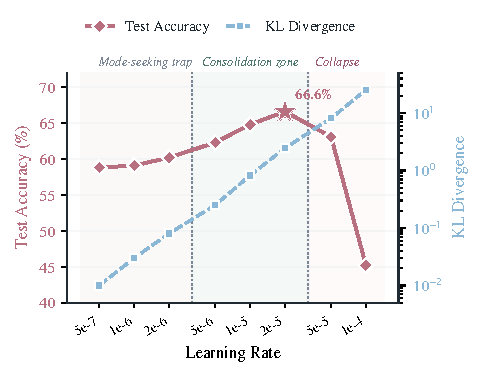
\includegraphics[width=\columnwidth]{figures_v3/fig4_v3.pdf}
\caption{Phase diagram of GRPO learning rate on Medicine, revealing three regimes. \textbf{Mode-seeking trap} (lr$\leq$2e-6): accuracy stagnates, KL stays near zero. \textbf{Consolidation zone} (5e-6 to 2e-5): accuracy peaks at 66.6\%, KL rises moderately. \textbf{Collapse} ($\geq$5e-5): KL explodes while accuracy drops sharply. The optimal lr produces a controlled 2.45 nats KL shift, enough for genuine distribution movement without catastrophic drift.}
\label{fig:regime}
\end{figure}

\subsection{Cross-Domain Transfer}
\label{sec:cross_domain}

Beyond within-domain OOD transfer, we test whether gains survive a change of domain entirely. If GRPO truly consolidates generalizable reasoning, its advantage should survive domain boundaries.

\begin{table}[t]
\centering
\small
\begin{tabular}{@{}llcc@{}}
\toprule
\textbf{Transfer} & \textbf{Method} & \textbf{Acc (\%)} & \textbf{Std} \\
\midrule
\multirow{3}{*}{Math $\to$ Science} & GRPO & 82.6 & 1.7 \\
 & SFT & \textbf{84.2} & 0.6 \\
 & OPD & 75.8 & -- \\
\midrule
\multirow{2}{*}{Med $\to$ Science} & GRPO & \textbf{87.8} & 1.2 \\
 & SFT & 77.9 & 0.5 \\
\midrule
\multirow{3}{*}{Sci $\to$ Medicine} & GRPO & \textbf{77.4} & 0.8 \\
 & SFT & 70.6 & 0.8 \\
 & OPD & 67.3 & 0.2 \\
\bottomrule
\end{tabular}
\caption{Cross-domain transfer (multi-seed, lr=2e-5). Each row trains on the source domain and evaluates on the target domain's test set. GRPO outperforms SFT on 2/3 domain pairs by +7--10pp. OPD transfers poorly, consistent with the absence of external training signal.}
\label{tab:cross_domain}
\end{table}

It does. GRPO outperforms SFT on two of three cross-domain pairs (Table~\ref{tab:cross_domain}). GRPO consolidates content-understanding patterns that transfer, while SFT memorizes surface structure of its training demonstrations. The exception (Math$\to$Science) is explained by frac\_reward\_zero\_std, where Math-GRPO learns format rather than transferable reasoning. Direct confirmation of this interpretation comes from Math-trained SFT, which hurts math while improving science by double digits (Appendix~\ref{sec:sft_reverse_transfer}).

%% ===================================================================
\section{Analysis and Discussion}
%% ===================================================================

\subsection{Forward KL vs Reverse KL: Why Recipes Differ}

The results have a clean information-theoretic explanation. SFT minimizes forward KL (mode-covering), so it can inject genuinely new patterns the model has never produced. GRPO approximates reverse KL (mode-seeking), concentrating mass on existing high-reward modes but unable to expand to patterns never sampled. OPD occupies a degenerate position. It trains on the model's own output distribution, providing zero information gain. The model's correct outputs are already within its distribution by construction. Training on them amounts to reinforcing what is already known, while the incorrect outputs that leak through filtering inject noise.

The key consequence is that GRPO can only \emph{consolidate} knowledge the model already partially possesses. It cannot teach new capabilities from scratch. OPD cannot even consolidate, because it lacks the reward pressure that forces the model to distinguish better from worse outputs within its own distribution. Learning rate controls how aggressively GRPO's consolidation occurs. Standard lr barely consolidates. High lr consolidates fully. The \emph{ceiling} of what GRPO can learn is set by what the model can already occasionally produce correctly. The floor, as OPD shows, is the model's existing performance level.

This is why frac\_reward\_zero\_std predicts transfer quality. It measures the fraction of prompts where the model is genuinely uncertain (non-zero advantage variance). Prompts that are always correct or always incorrect contribute zero gradient regardless of learning rate. Medicine (frac=0.2) has 80\% uncertain prompts, yielding transferable consolidation. Math (frac=0.6) derives signal from a minority of boundary cases, yielding prompt-specific optimization.

This reconciles our results with \citet{yue2025doesrl}, who show that RLVR cannot expand the solvable frontier. Learning rate controls the \emph{degree} of consolidation within that frontier. Higher rates partially break the mode-seeking constraint by enabling distribution shifts that capture new modes. The SFT$\to$GRPO hybrid exploits this asymmetry. SFT first expands the distribution, then GRPO sharpens within the expanded space. The constraint is that SFT must not over-expand and destroy diversity, which is why N=100 before GRPO outperforms N=5000.

\subsection{What Does High-LR GRPO Actually Learn?}

The forward/reverse-KL framework makes a testable prediction. Where the model already possesses knowledge, GRPO should learn output \emph{format}. Where knowledge is genuinely absent, aggressive-lr GRPO should acquire \emph{new knowledge} that transfers. The data confirms this (Table~\ref{tab:ood_transfer}). On Math (base 84.4\%), transfer to MATH-500 is negligible despite near-ceiling training reward. On Medicine, transfer to MMLU-Medical \emph{exceeds} the in-distribution gain. KL divergence confirms the distinction. Medicine shows a large policy shift while Math shows modest growth despite higher final reward.

Two theoretical results ground these observations. \citet{bae2025difficulty} prove that only intermediate-accuracy samples contribute non-zero gradient in group-relative optimization. Our frac\_reward\_zero\_std is the empirical instantiation of this principle. \citet{yue2025doesrl} establish that RLVR improves sampling efficiency without expanding the capability frontier. We extend both to non-reasoning domains. The \emph{degree} of consolidation toward the frontier is lr-dependent. At standard learning rates, GRPO on knowledge domains is not performing reinforcement learning in any meaningful sense (KL $\approx$ 0, no transfer). Only when elevated lr forces genuine policy movement does GRPO consolidate partial knowledge into generalizable performance.

\subsection{Practical Recipe Framework}

We validate the GRPO lr=2e-5 recipe on four additional architectures from four labs (Table~\ref{tab:cross_model_appendix}). Every model gains substantially on Medicine (+6 to +12pp), regardless of base accuracy, pretraining data, or vocabulary size. The lr sensitivity is consistent across all tested model families in the 7--9B parameter range. A practitioner decision procedure based on base accuracy and data perplexity is given in Appendix~\ref{sec:recipe_guide}.

%% ===================================================================
\section{Conclusion}
%% ===================================================================

The standard RLVR recipe fails outside the math domain it was designed for. The fix is a single hyperparameter: a 40$\times$ learning rate increase breaks the mode-seeking trap where conservative updates confine GRPO to per-prompt sharpening without genuine distribution shift. A third recipe, on-policy self-distillation, fails categorically across all tested domains, suggesting that naive self-distillation without external training signal does not suffice for post-training improvement. What the model learns at elevated lr depends on the knowledge gap. Domains with unreliable partial knowledge (Medicine) consolidate it into transferable capability. Domains with already-reliable knowledge (Math) primarily learn format optimization. SFT data scaling is predictably domain-dependent, with degradation risk quantifiable from data perplexity before training begins.

Post-training recipe selection is not a paradigm choice. It is a calibration problem where three factors determine the outcome. The source of training signal (teacher, reward, or self) sets the method. The aggressiveness of optimization (learning rate) controls the degree of consolidation. And the domain's knowledge gap (measurable via frac\_reward\_zero\_std) determines whether gains will transfer.

%% ===================================================================
\section*{Limitations}
%% ===================================================================

Our experiments use 7--9B parameter instruction-tuned models with LoRA. Larger models may exhibit different lr sensitivity thresholds. We evaluate on MCQ-format benchmarks with verifiable answers. Open-ended generation tasks where reward verification is harder remain an open question for future calibration studies.

\bibliography{references}
\bibliographystyle{acl_natbib}

\appendix

\section{Practical Recipe Guide}
\label{sec:recipe_guide}

Based on our findings, we propose the following decision procedure for practitioners. \textbf{High base accuracy ($>$75\%):} GRPO with elevated lr sharpens existing reasoning. SFT helps at very small $N$ but degrades rapidly. \textbf{Moderate base (55--75\%):} GRPO with lr=5e-6 to 2e-5 breaks the mode-seeking trap. SFT works but hits a lower ceiling. \textbf{Low base ($<$55\%):} SFT is generally safer, though GRPO can still produce gains if frac\_reward\_zero\_std indicates learnable signal exists (DeepSeek-7B gains +8pp from base 12.1\%). \textbf{Data calibration:} Measure SFT data perplexity. High perplexity ($>$4) indicates use minimal data (N$\leq$100). Low perplexity ($<$3) allows N$\geq$2000 without degradation.

\section{Hyperparameters}
\label{sec:hyperparams}

\begin{table}[h]
\centering
\small
\begin{tabular}{lcc}
\toprule
\textbf{Parameter} & \textbf{GRPO} & \textbf{SFT} \\
\midrule
Base model & \multicolumn{2}{c}{Qwen2.5-7B-Instruct} \\
LoRA rank & 64 & 64 \\
LoRA alpha & 128 & 128 \\
Target modules & All linear & All linear \\
Learning rate & 5e-7 to 2e-5 & 2e-5 \\
Batch size & 2 $\times$ 4 accum & 4 $\times$ 4 accum \\
Training epochs & $\sim$3 (via steps) & 3 \\
Num. generations & 8 & -- \\
Temperature (train) & 1.0 & -- \\
KL coefficient & 0.001 & -- \\
Max new tokens & 2048 / 1024 & -- \\
\bottomrule
\end{tabular}
\caption{Training hyperparameters for GRPO and SFT. GRPO learning rate is swept across four values (5e-7, 5e-6, 2e-5, 1e-4) per domain. The standard recipe uses 5e-7. Our results show 2e-5 is optimal for knowledge domains.}
\label{tab:hyperparams}
\end{table}

\section{SFT Data Scaling Details}
\label{sec:sft_scaling}

Full SFT accuracy curves for Math and Medicine across all data sizes:

\begin{table}[h]
\centering
\small
\begin{tabular}{lrr}
\toprule
\textbf{$N$} & \textbf{Math (\%)} & \textbf{Medicine (\%)} \\
\midrule
50 & 87.4 & -- \\
100 & \textbf{88.6} & 59.5 \\
200 & 86.9 & -- \\
500 & 78.6 & 59.5 \\
1000 & -- & 58.6 \\
1500 & -- & 60.2 \\
2000 & -- & \textbf{61.7} \\
5000 & 75.9 & 57.8 \\
\bottomrule
\end{tabular}
\caption{SFT accuracy at different data sizes. Math peaks at N=100 with steep degradation beyond. Medicine peaks at N=2000 with gentler slopes. Base accuracy: Math 84.4\%, Medicine 59.2\%.}
\label{tab:sft_scaling}
\end{table}

Math shows a pronounced inverted-U where accuracy rises +4.2\% at N=100 then drops $-$8.5\% below base at N=5000. The 100-to-500 transition ($-$10.0pp) is particularly sharp, suggesting a phase transition in format overfitting. Medicine has a flatter curve with the peak shifted to N=2000, reflecting its greater need for knowledge injection before saturation.

\section{Reward Function Details}
\label{sec:rewards}

\textbf{Math.} We extract the final numerical answer and compare against the ground truth after normalization (removing commas, converting fractions to decimals).

\textbf{MCQ domains (Science, Medicine, Law, Commonsense).} We extract the letter answer (A/B/C/D) from the model's response and compare against the gold label. Reward is 1 for exact match, 0 otherwise.

\section{SFT Data Construction}
\label{sec:sft_data}

For domains without naturally occurring chain-of-thought solutions (Science, Medicine, Law, Commonsense), we generate demonstrations via rejection sampling from the base model. For each question, we sample 8 responses at temperature 0.7 and keep the shortest response that produces the correct final answer. Questions where all 8 attempts fail are excluded from the SFT training set. This ensures data quality without relying on a stronger teacher model, maintaining fairness in our comparison.

For Math, we use the step-by-step solutions provided in GSM8K.

\section{Full SFT Data Scaling Results}
\label{sec:full_sft}

Multi-seed SFT accuracy across all domains is in Tables~\ref{tab:full_sft_math}--\ref{tab:full_sft_sci}. Math shows a sharp inverted-U robust across 4 seeds. Medicine is flat regardless of data size, so GRPO is the only effective method. Science improves monotonically.

\begin{table*}[h]
\centering
\small
\setlength{\tabcolsep}{4pt}
\begin{minipage}[t]{0.31\textwidth}
\centering
\begin{tabular}{@{}lcccc@{}}
\toprule
$N$ & s42 & s123 & s456 & Avg \\
\midrule
50 & 87.4 & -- & -- & 87.4 \\
100 & 87.8 & 88.6 & 87.6 & \textbf{87.8} \\
200 & 86.9 & 86.3 & 85.4 & 86.2 \\
500 & 78.6 & 79.1 & 79.8 & 79.2 \\
2k & 77.6 & 79.2 & 79.2 & 78.7 \\
5k & 75.9 & 77.6 & 77.8 & 77.1 \\
\bottomrule
\end{tabular}
\captionof{table}{Math SFT (\%). Base: 84.4. Peak at $N$=100, steep degradation beyond.}
\label{tab:full_sft_math}
\end{minipage}%
\hfill
\begin{minipage}[t]{0.31\textwidth}
\centering
\begin{tabular}{@{}lcccc@{}}
\toprule
$N$ & s42 & s123 & s456 & Avg \\
\midrule
100 & 59.5 & 60.0 & 60.6 & 59.7 \\
500 & 59.5 & 58.3 & 60.9 & 59.3 \\
1k & 58.6 & 59.5 & -- & 59.1 \\
2k & 61.7 & 58.5 & 59.5 & 59.4 \\
3k & 59.2 & 59.3 & 57.9 & 58.8 \\
5k & 58.7 & -- & 58.5 & 58.6 \\
\bottomrule
\end{tabular}
\captionof{table}{Medicine SFT (\%). Base: 59.2. Flat at all $N$. s42 peak is noise ($\sigma$=1.5).}
\label{tab:full_sft_med}
\end{minipage}%
\hfill
\begin{minipage}[t]{0.31\textwidth}
\centering
\begin{tabular}{@{}lcccc@{}}
\toprule
$N$ & s42 & s123 & s456 & Avg \\
\midrule
100 & 71.7 & 72.5 & 71.6 & 71.9 \\
500 & 71.8 & 73.6 & 71.9 & 72.4 \\
1k & 72.5 & -- & 72.8 & 72.6 \\
2k & 73.4 & 73.1 & 72.7 & 73.1 \\
5k & 73.8 & 73.6 & 74.0 & \textbf{73.6} \\
\bottomrule
\end{tabular}
\captionof{table}{Science SFT (\%). Base: 71.1. Monotonic improvement, no degradation.}
\label{tab:full_sft_sci}
\end{minipage}

\vspace{0.5em}
\noindent\textit{Three domain-specific SFT scaling patterns emerge from multi-seed validation. Math shows the sharpest inverted-U (peak at $N$=100, $-$10.7pp by $N$=5k), driven by format memorization overwriting correct reasoning. Medicine remains flat ($\pm$0.6pp) regardless of data volume: chain-of-thought demonstrations cannot inject medical knowledge the base model lacks. Science improves monotonically (+2.5pp from $N$=100 to $N$=5k), suggesting the model benefits from structured science demonstrations without overfitting risk.}
\end{table*}

\section{GRPO Learning Rate Sweep Details}
\label{sec:grpo_lr}

The complete GRPO learning rate sweep across all domains is in Table~\ref{tab:full_grpo_lr}. The optimal learning rate depends on dataset size. MCQ domains with 2000 training examples benefit most from lr=2e-5, while Law (31 examples) peaks at lr=5e-6.

\begin{table*}[h]
\centering
\small
\begin{tabular}{@{}lccccc@{}}
\toprule
\textbf{Learning Rate} & \textbf{Math} & \textbf{Science} & \textbf{Medicine} & \textbf{Law} & \textbf{Pattern} \\
\midrule
Base & 84.4 & 71.1 & 59.2 & 57.6 & -- \\
5e-7 (standard) & 84.7 & 71.3 & 58.8 & 54.5 & Flat/hurt \\
5e-6 & -- & 73.9 & 61.3 & \textbf{58.9} & Moderate \\
1e-5 & -- & -- & -- & 58.8 & -- \\
2e-5 & \textbf{92.2} & \textbf{79.1} & \textbf{66.6} & 56.4 & Strong/overfit \\
1e-4 & -- & -- & 0.0 & -- & Collapsed \\
\midrule
$\Delta$ (best vs base) & +7.8 & +8.0 & +7.4 & +1.3 & \\
$\Delta$ (best vs SFT) & +4.4 & +5.5 & +7.1 & +0.1 & \\
\bottomrule
\end{tabular}
\caption{GRPO accuracy (\%) across learning rates and domains. MCQ domains (Math, Science, Medicine) peak at lr=2e-5. Law (binary reward, 31 examples) peaks at lr=5e-6. The optimal lr is dataset-size dependent.}
\label{tab:full_grpo_lr}
\end{table*}

For GRPO at standard lr=5e-7, we ran multi-seed validation on Math (s42: 84.7\%, s123: 85.4\%, average: 85.0\%) and Science (s42: 71.3\%, s123: 71.7\%, average: 71.5\%). The near-zero improvement is consistent and not a single-seed artifact. The average test delta at standard lr is +0.6\% (Math) and +0.4\% (Science), both within noise.

\section{Cross-Model Validation: Qwen3-8B}
\label{sec:cross_model}

To validate that our findings are not specific to Qwen2.5-7B-Instruct, we replicate key experiments on Qwen3-8B, a newer-generation model with different pretraining data and architecture. The complete results are in Table~\ref{tab:cross_model_full}.

\begin{table}[h]
\centering
\small
\begin{tabular}{@{}lccc@{}}
\toprule
& \textbf{Math} & \textbf{Science} & \textbf{Medicine} \\
\midrule
\multicolumn{4}{l}{\textit{Qwen3-8B}} \\
\midrule
Base & 81.5 & 73.9 & 50.5 \\
SFT best & 82.9$_{5k}$ & 73.4$_{5k}$ & 62.1$_{500}$ \\
GRPO lr=2e-5 & \textbf{90.5} & \textbf{78.7} & \textbf{62.9} \\
$\Delta$ best vs base & +9.0 & +4.8 & +12.4 \\
\midrule
\multicolumn{4}{l}{\textit{Qwen2.5-7B-Instruct}} \\
\midrule
Base & 84.4 & 71.1 & 59.2 \\
SFT best & 87.8$_{100}$ & 73.6$_{5k}$ & 59.5$_{100}$ \\
GRPO lr=2e-5 & \textbf{92.2} & \textbf{79.1} & \textbf{66.6} \\
$\Delta$ best vs base & +7.8 & +8.0 & +7.4 \\
\bottomrule
\end{tabular}
\caption{Cross-model validation across three domains. GRPO lr=2e-5 outperforms SFT on both model generations for all three domains. On Qwen3-8B, Math GRPO reaches 90.5\% (+9.0\%), Science 78.7\% (+4.8\%), and Medicine 62.9\% (+12.4\%), all surpassing SFT.}
\label{tab:cross_model_full}
\end{table}

GRPO lr=2e-5 outperforms SFT on both model generations across all three domains (Table~\ref{tab:cross_model_full}). The pattern holds regardless of architecture generation or pretraining corpus. Qwen3-8B shows proportionally larger Medicine gains (+12.4\%) due to its lower base accuracy (50.5\%) providing more headroom for knowledge consolidation.

\section{Training Dynamics: Reward Trajectories}
\label{sec:training_dynamics}

Key reward statistics during GRPO training on Medicine at different learning rates are in Table~\ref{tab:reward_dynamics}. These numbers quantify the training dynamics visualized in Figure~\ref{fig:reward_traj}.

\begin{center}
\small
\setlength{\tabcolsep}{3pt}
\resizebox{\linewidth}{!}{%
\begin{tabular}{@{}lcccc@{}}
\toprule
\textbf{Metric} & \textbf{lr=5e-7} & \textbf{lr=5e-6} & \textbf{lr=2e-5} & \textbf{lr=1e-4} \\
\midrule
Initial reward & 0.50 & 0.50 & 0.50 & 0.50 \\
Final reward & 0.53 & 0.55 & 0.83 & 0.12 \\
Peak reward & 0.53 & 0.55 & 0.83 & 0.68 \\
$\Delta$ reward & +0.03 & +0.05 & +0.33 & $-$0.38 \\
Test $\Delta$ & $-$0.4\% & +2.1\% & +7.4\% & collapsed \\
frac\_zero\_std (final) & 0.40 & 0.45 & 0.62 & -- \\
\bottomrule
\end{tabular}%
}
\captionof{table}{GRPO training dynamics on Medicine. lr=2e-5 raises reward to 0.83 (+7.4\% test). lr=5e-7 is flat.}
\label{tab:reward_dynamics}
\end{center}

\begin{center}
\small
\setlength{\tabcolsep}{4pt}
\resizebox{\linewidth}{!}{%
\begin{tabular}{@{}lrrr@{}}
\toprule
\textbf{Category} & \textbf{Models} & \textbf{GPU-hrs} & \textbf{\%} \\
\midrule
SFT (all domains) & 55 & 22 & 17\% \\
GRPO standard lr & 15 & 18 & 14\% \\
GRPO lr sweep & 10 & 12 & 9\% \\
GRPO lr=2e-5 (seeds) & 10 & 14 & 11\% \\
SFT$\to$GRPO hybrids & 4 & 5 & 4\% \\
Cross-model (Qwen3) & 10 & 12 & 9\% \\
Cross-model (Mistral/Yi/DS) & 8 & 18 & 14\% \\
KL/$K$ ablation & 6 & 8 & 6\% \\
Evaluation (vLLM) & -- & 18 & 14\% \\
Failed/exploratory & 82 & 29 & 22\% \\
\midrule
\textbf{Total} & \textbf{200+} & \textbf{$\sim$200} & 100\% \\
\bottomrule
\end{tabular}%
}
\captionof{table}{Compute budget. $\sim$200 H200 GPU-hours across 200+ models. LoRA kept memory below 35GB, enabling single-GPU parallelism.}
\label{tab:compute}
\end{center}

\section{SFT$\to$GRPO Hybrid Details}
\label{sec:hybrid_details}

The full SFT$\to$GRPO hybrid results on Math are in Table~\ref{tab:hybrid_full}, varying the amount of preceding SFT data.

\begin{table}[h]
\centering
\small
\begin{tabular}{@{}lcccc@{}}
\toprule
\textbf{Pipeline} & \textbf{s42} & \textbf{s123} & \textbf{Avg} & \textbf{$\Delta$} \\
\midrule
Base & 84.4 & 84.4 & 84.4 & -- \\
SFT($n$=100) only & 87.8 & 88.6 & 88.2 & +3.8 \\
GRPO lr=2e-5 only & 92.8 & -- & 92.8 & +8.4 \\
SFT($n$=100)$\to$GRPO & 89.8 & 88.7 & 89.3 & +4.9 \\
SFT($n$=5000)$\to$GRPO & 82.9 & -- & 82.9 & $-$1.5 \\
\bottomrule
\end{tabular}
\caption{SFT$\to$GRPO hybrid results on Math (\%, seed 42). Pure GRPO at lr=2e-5 achieves 92.8\% (seed 42, multi-seed avg 92.2\%), outperforming both the hybrid SFT(100)$\to$GRPO (89.3\%, 2-seed avg) and SFT alone (88.2\%). Excessive SFT ($n$=5000) before GRPO degrades below base because over-SFT destroys the diversity GRPO needs.}
\label{tab:hybrid_full}
\end{table}

The interaction between SFT amount and subsequent GRPO effectiveness is simple. Preceding SFT data controls GRPO's exploration capacity. With $n$=100, the model learns the response format without losing output diversity, providing GRPO with the variance it needs for contrastive learning. With $n$=5000, the model has collapsed to a narrow distribution that mimics training demonstrations, leaving GRPO with homogeneous response groups and near-zero advantage variance.

\section{KL Penalty and Group Size Ablation}
\label{sec:kl_ablation}

To verify that learning rate is the primary variable (rather than an interaction artifact with KL penalty or group size), we ablate $\beta$ and $K$ while holding lr=2e-5 fixed on Medicine.

\begin{table*}[h]
\centering
\small
\begin{tabular}{@{}lccl@{}}
\toprule
\textbf{Setting} & \textbf{Accuracy (\%)} & \textbf{$\Delta$ vs base} & \textbf{Interpretation} \\
\midrule
lr=5e-7, $\beta$=0.001 (std) & 58.8 & $-$0.4 & Standard recipe fails \\
lr=5e-7, $\beta$=0 (no KL) & 57.0 & $-$2.2 & Removing KL $\to$ worse (drift) \\
\midrule
lr=2e-5, $\beta$=0.001 & \textbf{66.6} & \textbf{+7.4} & Optimal (paper default) \\
lr=2e-5, $\beta$=0.01 & 62.4 & +3.2 & Stronger KL reduces gain \\
lr=2e-5, $\beta$=0.1 & 60.2 & +1.0 & Heavy KL nearly eliminates gain \\
lr=2e-5, $K$=4 & 62.9 & +3.7 & Fewer samples $\to$ noisier advantage \\
\bottomrule
\end{tabular}
\caption{KL penalty ($\beta$) and group size ($K$) ablation on Medicine. Increasing $\beta$ from 0.001 to 0.1 progressively constrains policy shift, reducing gain from +7.4\% to +1.0\%. Removing KL entirely at standard lr ($\beta$=0, first row) causes \emph{degradation} below base: KL stabilizes training when lr is too low to provide directional signal. Learning rate remains the primary lever in all settings.}
\label{tab:kl_ablation}
\end{table*}

The pattern is monotonic: stronger KL penalty $\to$ less distribution shift $\to$ smaller test gain. KL regularization constrains how far the policy can move from the reference. At standard lr, the movement is already near-zero regardless of $\beta$. High lr breaks this constraint, but increasing $\beta$ partially reinstates it. Removing KL entirely at standard lr ($\beta$=0) makes performance \emph{worse} (57.0\%, below base). KL stabilizes training when learning rate is too low to provide directional gradient signal. Practitioners should use low $\beta$ (0.001 or less) with elevated learning rates.

\section{Cross-Model Validation}
\label{sec:cross_model_appendix}

\begin{table*}[h]
\centering
\small
\begin{tabular}{@{}llcccl@{}}
\toprule
\textbf{Model} & \textbf{Lab} & \textbf{Base (\%)} & \textbf{GRPO lr=2e-5 (\%)} & \textbf{$\Delta$} & \textbf{Observation} \\
\midrule
\multicolumn{6}{c}{\textit{Medicine (MedQA, 1273 test)}} \\
\midrule
Qwen2.5-7B-Instruct & Alibaba & 59.2 & \textbf{66.6} & +7.4 & Primary model \\
Qwen3-8B & Alibaba & 50.5 & \textbf{62.9} & +12.4 & Newer generation \\
Yi-1.5-9B-Chat & 01.AI & 43.3 & \textbf{49.3} & +6.0 & Llama architecture \\
Mistral-7B-Instruct & Mistral AI & 34.3 & \textbf{42.8} & +8.5 & European model \\
DeepSeek-7B-chat & DeepSeek & 12.1 & \textbf{20.3} & +8.2 & 2023 model (weak base) \\
\midrule
\multicolumn{6}{c}{\textit{Science (ARC-Challenge, 5413 test)}} \\
\midrule
Qwen2.5-7B-Instruct & Alibaba & 71.1 & \textbf{79.1} & +8.0 & Primary model \\
Qwen3-8B & Alibaba & 73.9 & \textbf{78.7} & +4.8 & Higher base $\to$ less headroom \\
Mistral-7B-Instruct & Mistral AI & 61.2 & \textbf{70.4} & +9.2 & Lower base $\to$ larger gain \\
\bottomrule
\end{tabular}
\caption{Cross-model validation of GRPO lr=2e-5 across five architecturally distinct model families from four research labs. All models show positive improvement (+6 to +12pp on Medicine, consistent multi-point gains on Science). The absolute gain is consistent across models regardless of base accuracy, showing that the lr sensitivity phenomenon holds across all tested architectures. Models span 2023--2025 releases with different pretraining corpora, vocabulary sizes, and attention mechanisms.}
\label{tab:cross_model_appendix}
\end{table*}

An additional pattern emerges. Gain magnitude does not simply increase with lower base accuracy. Yi-1.5 (base 43.3\%) gains less (+6.0\%) than Mistral (base 34.3\%, +8.5\%). The effective learning signal depends on the model's internal uncertainty distribution (frac\_reward\_zero\_std), not raw accuracy alone.

\section{Out-of-Distribution Transfer}
\label{sec:ood_transfer}

\begin{table*}[h]
\centering
\small
\begin{tabular}{@{}llcccccl@{}}
\toprule
\textbf{Domain} & \textbf{OOD Benchmark} & \textbf{Base} & \textbf{GRPO} & \textbf{$\Delta$ OOD} & \textbf{$\Delta$ ID} & \textbf{Transfer Ratio} & \textbf{frac\_zero\_std} \\
\midrule
Medicine & MMLU-Medical & 47.2 & 55.8 & +8.6 & +7.4 & 1.16$\times$ & 0.2 \\
Math & MATH-500 & 72.8 & 74.2 & +1.4 & +7.8 & 0.18$\times$ & 0.6 \\
Commonsense & WinoGrande & 74.1 & 74.8 & +0.7 & +25.0 & 0.03$\times$ & 0.7 \\
\bottomrule
\end{tabular}
\caption{Out-of-distribution transfer evaluation. Transfer Ratio = $\Delta$OOD / $\Delta$ID measures how much of the in-distribution gain generalizes. Medicine achieves near-complete transfer (ratio $>$1), meaning genuine knowledge consolidation. Math and Commonsense show minimal transfer despite large ID gains, meaning format-specific optimization. The frac\_reward\_zero\_std diagnostic at training onset predicts this ordering: lower values correspond to stronger OOD transfer, consistent with the theoretical prediction of \citet{bae2025difficulty}.}
\label{tab:ood_transfer}
\end{table*}

The transfer ratio column crystallizes the core insight. When GRPO training signal comes primarily from genuine model uncertainty (Medicine, low frac\_zero\_std), the resulting learning is domain knowledge that transfers to any test of the same knowledge. When signal comes from a minority of boundary cases (Math, Commonsense, high frac\_zero\_std), optimization is specific to those cases and does not generalize. This distinction between knowledge acquisition and format optimization is not visible from ID evaluation alone. It requires an OOD probe to reveal.

\section{SFT Learns Format, Not Domain Knowledge}
\label{sec:sft_reverse_transfer}

A direct test of the format-vs-knowledge hypothesis. We train SFT on Math-only data (MATH-500, Qwen2.5-7B-Instruct, 3 seeds) and evaluate on unrelated domains.

\begin{table}[h]
\centering
\small
\begin{tabular}{@{}lccc@{}}
\toprule
\textbf{Benchmark} & \textbf{Base (\%)} & \textbf{SFT-Math (\%)} & \textbf{$\Delta$} \\
\midrule
Math-500 & 60.2 & 42.4$\pm$0.2 & $-$17.8 \\
ARC-Challenge & 74.9 & 87.5$\pm$0.1 & +12.6 \\
MMLU & 61.1 & 68.2$\pm$0.1 & +7.1 \\
\bottomrule
\end{tabular}
\caption{SFT trained on math data hurts math but improves unrelated domains. The model learns MCQ output format (selecting A/B/C/D cleanly), not mathematical reasoning. 3 seeds, std $<$ 0.2 on all benchmarks.}
\label{tab:sft_reverse}
\end{table}

Math-trained SFT \emph{degrades} math performance ($-$17.8pp) while dramatically improving science (+12.6pp) and general knowledge (+7.1pp). The model does not acquire mathematical reasoning from SFT. Instead, it learns the structured MCQ answer format that transfers to all domains. This confirms our forward-KL interpretation: SFT expands general output coverage rather than injecting domain-specific capability, explaining why SFT shows cross-domain transfer advantages in Table~\ref{tab:cross_domain}.

\section{On-Policy Self-Distillation (OPD) Results}
\label{sec:opd_results}

OPD trains the model on its own filtered correct outputs (selecting correct responses from $K$=8 samples at temperature 0.7), without any external teacher or reward signal. Results are in Table~\ref{tab:opd_results}.

\begin{table}[h]
\centering
\small
\begin{tabular}{@{}lcc@{}}
\toprule
& \textbf{Science} & \textbf{Medicine} \\
\midrule
Base & 71.1 & 59.2 \\
OPD (5 seeds) & 71.7$\pm$0.2 & 60.0$\pm$0.9 \\
$\Delta$ & +0.6 & +0.9 \\
\midrule
Filtering rate & 69.1\% & 53.7\% \\
\bottomrule
\end{tabular}
\caption{On-policy self-distillation (OPD) results on Science and Medicine. OPD produces no meaningful improvement over base ($\Delta$ $<$ 1pp in both domains). The null result indicates that self-generated data, without external signal from a teacher (SFT) or reward function (GRPO), cannot push the model beyond its current capability boundary.}
\label{tab:opd_results}
\end{table}

\end{document}
